%%%%%%%%%%%%%%%%%%%%%%%%%%%%%%%%%%%%%%%%%%%%%%%%%%%%%%%%%%
%
% Vzor pro sazbu kvalifikační práce
%
% Západočeská univerzita v Plzni
% Fakulta aplikovaných věd
% Katedra informatiky a výpočetní techniky
%
% Petr Lobaz, lobaz@kiv.zcu.cz, 2016/03/14
%
%%%%%%%%%%%%%%%%%%%%%%%%%%%%%%%%%%%%%%%%%%%%%%%%%%%%%%%%%%

% Možné jazyky práce: czech, english
% Možné typy práce: BP (bakalářská), DP (diplomová)
\documentclass[czech,BP]{thesiskiv}

% Definujte údaje pro vstupní strany
%
% Jméno a příjmení; kvůli textu prohlášení určete, 
% zda jde o mužské, nebo ženské jméno.
\author{Přemysl Oráč}
\declarationmale

%alternativa: 
%\declarationfemale

% Název práce
\title{Titul práce\\nanejvýš na dvě\\až tři řádky}

% 
% Texty abstraktů (anglicky, česky)
%
\abstracttexten{The text of the abstract (in English). It contains the English translation of the thesis title and a short description of the thesis.}

\abstracttextcz{Text abstraktu (česky). Obsahuje krátkou anotaci (cca 10 řádek) v češtině. Budete ji potřebovat i při vyplňování údajů o bakalářské práci ve STAGu. Český i anglický abstrakt by měly být na stejné stránce a měly by si obsahem co možná nejvíce odpovídat (samozřejmě není možný doslovný překlad!).
}

% Na titulní stranu a do textu prohlášení se automaticky vkládá 
% aktuální rok, resp. datum. Můžete je změnit:
%\titlepageyear{2016}
%\declarationdate{1. března 2016}

% Ve zvláštních případech je možné ovlivnit i ostatní texty:
%
%\university{Západočeská univerzita v Plzni}
%\faculty{Fakulta aplikovaných věd}
%\department{Katedra informatiky a výpočetní techniky}
%\subject{Bakalářská práce}
%\titlepagetown{Plzeň}
%\declarationtown{Plzni}

%%%%%%%%%%%%%%%%%%%%%%%%%%%%%%%%%%%%%%%%%%%%%%%%%%%%%%%%%%
%
% DODATEČNÉ BALÍČKY PRO SAZBU
% Jejich užívání či neužívání záleží na libovůli autora 
% práce
%
%%%%%%%%%%%%%%%%%%%%%%%%%%%%%%%%%%%%%%%%%%%%%%%%%%%%%%%%%%

% Zařadit literaturu do obsahu
\usepackage[nottoc,notlot,notlof]{tocbibind}

% Umožňuje vkládání obrázků
\usepackage[pdftex]{graphicx}

% Odkazy v PDF jsou aktivní; navíc se automaticky vkládá
% balíček 'url', který umožňuje např. dělení slov
% uvnitř URL
\usepackage[pdftex]{hyperref}
\hypersetup{colorlinks=true,
  unicode=true,
  linkcolor=black,
  citecolor=black,
  urlcolor=black,
  bookmarksopen=true}

% matematicke rovnice %
\usepackage{amsmath}

% Při používání citačního stylu csplainnatkiv
% (odvozen z csplainnat, http://repo.or.cz/w/csplainnat.git)
% lze snadno modifikovat vzhled citací v textu
\usepackage[numbers,sort&compress]{natbib}

%%%%%%%%%%%%%%%%%%%%%%%%%%%%%%%%%%%%%%%%%%%%%%%%%%%%%%%%%%
%
% VLASTNÍ TEXT PRÁCE
%
%%%%%%%%%%%%%%%%%%%%%%%%%%%%%%%%%%%%%%%%%%%%%%%%%%%%%%%%%%
\begin{document}
%
\maketitle
\tableofcontents

\chapter{Úvod}
V souboru \texttt{literatura.bib} jsou uvedeny příklady, jak citovat knihu \cite{KnuthAOCP2}, článek v časopisu \cite{Hoare1961}, webovou stránku \cite{Graphics2D}.


\chapter{Úvod}
V dnešní době, kdy je svět přesycen obrázky v digitální podobě, není vůbec snadné nalézt obrázek zobrazující požadovaný obsah. Naneštěstí počítače nedokáží vnímat obraz jako lidé, vnímají totiž obrazy jako sérii binárních informací. Přitom počítače a jejich práce s obrazy by se dala využít v mnoha oborech jako je lékařství nebo doprava. Na základě toho vyplouvá na povrch problém jak spravovat digitální obrázky a efektivně mezi nimi vyhledávat. Prostřednictvím klíčových slov přiřazených k obrázkům se dá problém vyhledávání zjednodušit. Přiřazení klíčových slov probíhá pomocí procesu automatické anotace obrázků. Klíčová slova přiřazená k obrázku by měla vyjadřovat jeho obsah (například les, strom). Při reálném použití můžeme ovšem narazit na problém při zadávání abstraktních slov, například šťastná rodina.  
\\
Pro automatickou anotaci obrázků se používá strojové učení. Můžeme ji rozdělit na dvě části. V první části získáme klíčové příznaky ve druhé už je samotná anotace, tedy přidělení klíčových slov. Abychom tento postup mohli provést v praxi, musíme nejdřív klasifikátor natrénovat pomocí trénovací množiny. Trénovací množina je množina obrázků, která již má ke každému obrázku přidána metadata s klíčovými slovy připravenými od lidí. Vybrané obrázky v trénovací množině musí být různorodé, aby anotace probíhala správně. Pojem automatická anotace obrázků je jednoduše řečeno proces, při kterém jsou k obrázku automaticky přiřazena metada, která obsahují klíčová slova. 
\\
Cílem práce je navrhnout a implementovat software umožňující automatickou anotaci obrázků. Konkrétně se bude zabývat metodou JEC. Práce bude využívat nízkoúrovňové příznaky, konkrétně barvu a texturu. Metodu budeme zkoušet na standardních datech, následně se budeme snažit výsledky vylepšít, a porovnat s další metodou a literaturou.


\chapter{JEC Joint Equal Contribution}
Tato metoda je založena na hypotéze, že podobné obrázky mají podobná klíčová slova. Pomocí metody hledání nejbližších sousedů (dále jen KNN) najdeme K nejpodobnějších obrázků. Přičemž klíčová slova od jednotlivých sousedů jsou posuzována odlišně a to právě na základě toho o kolik se s testovaným obrázkem liší. Metoda je postavena na dvou typech příznaků - barevných a texturových. 


\section{Příznaky}
Barva a textura jsou považovány za dva nejdůležitější nizkoúrovňové příznaky pro obrázkovou reprezentaci. Nejběžnější barevné deskriptory jsou barevné histogramy, které jsou často využívány pro porovnávání a indexování obrázků, zejména z důvodu jejich efektivnosti a snadného výpočtu. K vytvoření texturových příznaků se používají Haarovy a Gaborovy wavelety a to především z důvodu že jsou efektivní při vytváření rozptýlených diskriminativních obrázkových rysů.  

\subsection{Barva}
U digitálního obrazu je barva reprezentovaná n-rozměrným vektorem. Jeho velikost a význam jednotlivých složek (tzv. barevných kanálů) zavisí na příslušném barevném prostoru. Počet bitů použitých k uložení buď celého vektoru nebo jeho jednotlivých složek se nazývá barevná hloubka (totožně bitová hloubka). Obvykle se můžeme setkat s hodnotami 8, 12, 14 a 16 bitů na kanál. 
\\
V použité metodě získáme vlastnosti z obrázků ve třech rozdílných barevných prostorech: RGB, HSV a LAB. RGB (Red, Green, Blue) je nejobvykleji používaný pro zachycení obrázu nebo jeho zobrazení. Oproti tomu HSV (Hue, Saturation and Value) se snaží zachytit barevný model tak jak ho vnímá lidské oko, ale zároveň se snaží zůstat jednoduchý na výpočet. Hue znamená odstín barvy, saturation systost barvy a value je hodnota jasu nebo také množství bílého světla. RGB je závislý na konkrétním zařízení, nemůže dosáhnout celého rozsahu barev, které vidí lidské oko, zatímco barevný model LAB je shopen obsáhnout celé viditelné spektrum a navíc je nezávislý na zařízení. L (ve zkratce LAB) značí Luminanci (jas dosahuje hodnot 0 - 100, kde 0 je černá a 100 je bílá). Zbylé A a B jsou dvě barvonosné složky, kdy A je ve směru červeno/zeleném a B se pohybuje ve směru modro/žlutém. 


Pro RGB, HSV i LAB použijeme barevnou hloubku 16 bitů na kanál histogramu v jejich příslušném barevném prostoru. 

Jako reprezentace textur budou použity Gabor a Haar wavelety. Každý obrázek bude filtrován s Gabor wavelet na třech škálách a čtyřech orientacích. 

\section{Vzdálenosti}
 K určení příslušné vzdálenosti se můžeme setkat se čtyřmi měřítky vzdálenosti pro histogramy a rozdělení (K L-divergence, $\chi^2$ statistika, L1 - vzdálenost a L2 - vzdálenost). Na RGB a HSV je nejlépší použít L1 zatímco pro LAB je nejvhodnější K L-divergence. 
 
\section{Textura}
Gabor filter je lineární filter používaný pro detekci hran. Frekvence a orientace reprezentující Gabor filter je podobná lidskému vnímání a jsou zvláště vhodné pro reprezentaci textury a rozlišování. 

TODO Dohledat Haar a Gabor wavelety, přidat vzorečky a zase klidně i obrázky


\section{Přenesení klíčových slov}
Pro přenesení klíčových slov používáme metodu, kdy přeneseme n klíčových slov k dotazovanému obrázku $\tilde{I}$ od K nejbližších sousedů v trénovací sadě. Mějme $I_{i}, i = 1, ..., K$ ,tyto K nejbližší sousedy seřadíme podle vzrůstající vzdálenosti (tzn. že $I_{1} $ je nejvíce podobný obrázek). Počet klíčových slov k danému $I_{i}$ je označen jako $|I_{i}|$. Dále jsou popsány jednotlivé kroky alogoritmu na přenesení klíčových slov.
\begin{enumerate}
	\item Seřadíme klíčová slova z $I_{1}$ podle jejich frekvence v trénovacích datech.
	\item Z $|I_{1}|$ klíčových slov z $I_{1}$ přeneseme n nejvýše umístěná klíčová slova do dotazovaného $\tilde{I}$. Když $|I_{1}| < n$ pokračujte na krok 3. 
	\item Seřaď klíčová slova sousedů od $I_{2}$ do $I_{K}$ podle dvou faktorů
	\begin{enumerate}
		\item Co výskyt v trénovacích datech s klíčovými slovy přenesených v kroku 2 a
		\item místní frekvence (tj. jak často se vyskytují jako klíčová slova u obrázků $I_{2}$ až $I_{K}$). Vyber nejvyšší rankink $n-|I_{1}|$ klíčových slov převedených do $\tilde{I}$.
	\end{enumerate}
\end{enumerate}

Tento algoritmus pro přenos klíčových slov je poněkud odlišný od algoritmů které se běžně používají. Jeden z běžně užívaných funguje na principu, že klíčová slova jsou vybrána od všech sousedů (se všemi sousedy je zacházeno stejně bez ohledu na to jak jsou danému obrázku podobní), jiný užívaný algoritmus k sousedům přistupuje váženě (každý soused má jinou váhu)a to na základě jejich vzdálenosti od testovaného obrázku. Při testování se ovšem ukázalo, že tyto přímé přístupy přináší horší výsledky v porovnání s použitým dvoufaktorovým algoritmem pro přenos klíčových slov. \\
V souhrnu použitá metoda je složenina ze svou složeniny obrázkové vzdálenosti měřítku (JEC nebo Lasso) pro nejbližší ranking, kombinuje se s výše popsaným algoritmem na přenášení klíčových slov.

\chapter{Testovací databáze}
Pro natrénování a následné testování byla použita data z databází ČTK, ESP a IAPRC.

\section{ČTK}
Data od ČTK obsahují 3 383 obrázků. Ke každému obrázku jsou přidána metadata ve formátu XML, která obsahují klíčová slova a další informace o obrázku. 

\section{ESP}
Data od ESP obsahují 67 796 obrázků ve formátu jpg. Ke každému obrázku je přiřazen soubor ve formátu desc, který obsahuje anglické anotace.

\begin{figure}[h]
		\centering
		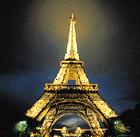
\includegraphics[width=140px]{./img/ESP.jpg}	
		\caption{Ukázka obrázku s klíčovými slovy: tower, france, high, gold, paris, yellow, night, light, black, eiffel, dark}
\end{figure}

\section{iaprtc12}
Data iaprtc12 obsahují 13 031 obrázků ve formátu jpg. Ke každému obrázku jsou přiložena metadata ve formátu XML, která obsahují 
infromace o obrázku v různých jazycích. Kromě angličtiny je tam i například španělština nebo němčina. V metadatatech ovšem nenajdeme klíčová slova tak jak by jsme si je představovali, ale v různých tagách nalezneme například titulek obrázku, který může vypadat například The Plaza de Armas, a v tagu description je například  a woman and a child are walking over the square.


\chapter{Návrh systému}
Systém byl navržen jako modulový a to z důvodu snadné obměny některé z častí, což je výhodné zejména pokud bychom potřebovali například spočítat vzdálenosti vektorů podle jiného algoritmu. 

\begin{figure}[h]
		\centering
		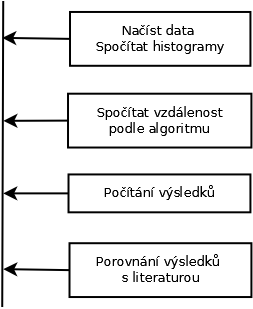
\includegraphics[width=253px]{./img/graf.png}	
		\caption{Návrh systému}
\end{figure}


\chapter{Použité programové prostředky}
Program byl navržen na operační systému Linux. Jako programovací jazyk byl zvolen Python a to z důvodu jeho jednoduchého použití, což je na prototyp, jako je tento velice výhodné na časovou náročnost. Program využívá knihovnu OpenCV 3.1. 
  
\section{OpenCV}
OpenCV (Open source computer vision) je knihovna vydávána pod licencí BSD a je volně k dispozici jak pro akademické účely, tak pro komerční použití. Je vhodná pro použití v C++, C, Python a Javě. Podporuje operační systémy Windows, Linux, Mac OS, iOS a Android.
\\
Knihovna byla navrhnuta pro výpočetní efektivitu v oblasti počítačového vidění a zpracování obrazu se zaměřením na zpracování obrazu v reálném čase. Z důvodu optimalizace byla napsána v C/C++. 
\\
Knihovnu OpenCV je možné stáhnout na adrese: http://opencv.org/


\chapter{Vyhodnocení výsledků}
Zpracování výsledků probíhá jako porovnání anotací přidělených člověkem s anotacemi přidělenymi klasifikátorem. Označme si $w_auto$ jako počet obrázků, kterým bylo dané slovo přiřazeno klasifikátorem, $w_human$ počet obrázků kterým bylo dané slovo přiřazeno člověkem. U klasifikátorů se počítá precision (přesnost) a recall (úplnost) pro každé slovo v testovací sadě.\\
Recall \eqref{recall} je počet obrázků správsně anotovaných s daným slovem děleno počtem obrázků kterým bylo toto slovo přiděleno v anotaci člověkem. Precision \eqref{precision} je počet správně anotovaných obrázků s tímto slovem děleno celkovým počtem anotovaných obrázků s tímto slovem(správně nebo ne). 
\begin{align}
   \label{recall} Rec = \frac{w_c}{w_h}
\end{align}
\begin{align}
   \label{precision} Prec = \frac{w_c}{w_a}
\end{align}


\chapter{Závěr}
V teoretické části byly popsány nízkoúrovňové příznaky barva a textura. Byla rozebrána metoda JEC, která bude v bakalářské práci implementována. Seznámili jsme se s knihovnou OpenCV, prostudovali obrázky a přiložená metadata od ČTK, ESP a iaprtc12. 

\chapter{Uživatelská dokumentace}
popsani jak vypada zdrojovej soubor kterej to zere, nejdriv cesta k souboru a pak jeho klicovy slova
 
% 
% PRO ANGLICKOU SAZBU JE NUTNÉ ZMĚNIT
% CITAČNÍ STYL!
%
\bibliographystyle{csplainnatkiv}
{\raggedright\small
\bibliography{literatura}
}

\end{document}
